\problemname{Samla stenar}

$N$ stenar ligger stökigt utspridda i ett koordinatsystem. Varje sten har en koordinat ($x_i$,$y_i$). Det har blivit dags att samla ihop stenarna, och till din hjälp har du skaffat en supersmart stenplockarmaskin.

Innan maskinen startar så ska du välja en punkt som du kallar uppsamlingspunkten $S$. Det är punkten där maskinen börjar, och där den kommer att placera de insamlande stenarna. Den måste ligga någonstans på x-axeln. Maskinen börjar på uppsamlingspunkten $(S,0)$, och samlar sedan upp alla stenar och placerar dem på uppsamlingspunkten. Maskinen kan bara bära \emph{en sten i taget}.

Bränsle är dyrt, så du tänkte försöka vara lite smart. Du vet att när maskinen sätter igång så åker den alltid och samlar upp alla stenar på optimalt vis, men de är upp till dig att välja uppsamlingspunkten så att den totala sträckan maskinen åkt blir minimal. Hur lång blir denna sträcka, givet att du väljer uppsamlingspunkten optimalt? Du kan betrakta stenarna och maskinen som punkter i talplanet.

\section*{Indata}
Den första raden innehåller heltalet $N$ ($1 \leq N \leq 10^5$), antalet stenar.

Sedan följer $N$ rader med par av flyttal $x_i y_i$, stenarnas koordinater. Alla stenar i
indata ligger maximalt 100 längdenheter från origo.

\section*{Utdata}
Skriv ut ett heltal: minsta möjliga totala sträcka som maskinen har åkt efter att den samlat upp alla stenar. Ett absolut fel mindre än $10^{-4}$ betraktas som korrekt.

{\bf Tips:} Se till att ditt program skriver ut tillräckligt många decimaler även när svaret är stort.

\section*{Poängsättning}
Din lösning kommer att testas på en mängd testfallsgrupper.
För att få poäng för en grupp så måste du klara alla testfall i gruppen.

\noindent
\begin{tabular}{| l | l | p{12cm} |}
  \hline
  \textbf{Grupp} & \textbf{Poäng} & \textbf{Gränser} \\ \hline
  $1$    & $30$       & Alla stenar ligger på x-axeln och $N \leq 1000$. \\ \hline
  $2$    & $30$       & Alla stenar ligger på x-axeln. \\ \hline
  $3$    & $40$       & Inga ytterligare begränsningar. \\ \hline
\end{tabular}


\section*{Förklaring till exempel 1}

\begin{figure}[!h]
\begin{center}
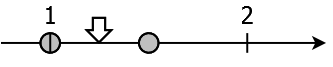
\includegraphics[scale=0.4]{stenar1.png}
\end{center}
\caption{Figuren visar ett möjligt val på startpunkt som leder till minimal körsträcka för maskinen, x = 1.25. Maskinen behöver åka 0.5 längdenheter för att hämta den vänstra stenen, och sedan 0.5 längdenheter för att hämta den högra.}
\label{fig1}
\end{figure}

\section*{Förklaring till exempel 2}
\begin{figure}[!h]
\begin{center}
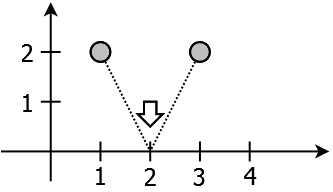
\includegraphics[scale=0.4]{stenar2.png}
\end{center}
\caption{Figuren visar den optimala startpositionen för maskinen, vid x = 2.0. Total sträcka åkt blir $4\cdot\sqrt{2^2 + 1} = 8.94427191...$ .}
\label{fig1}
\end{figure}
